%% 
%% Supplementary Material -- Article 2
%% Biocultural Vulnerability in Traditional Agricultural Knowledge
%%

\documentclass[12pt,a4paper]{article}

%% Packages
\usepackage{amssymb}
\usepackage{amsmath}
\usepackage{bm}
\usepackage[utf8]{inputenc}
\usepackage[T1]{fontenc}
\usepackage{booktabs}
\usepackage{graphicx}
\graphicspath{{../../}}
\usepackage{float}
\usepackage{hyperref}
\usepackage{natbib}
\usepackage{geometry}
\geometry{margin=2.5cm}
\usepackage{setspace}
\onehalfspacing

\begin{document}

\title{Supplementary Material\\[0.5em]
\large Biocultural vulnerability in Traditional Agricultural Knowledge: a quantitative meta-analysis}

\author{Catuxe Varj\~ao de Santana Oliveira \and Luiz Diego Vidal Santos}

\date{}
\maketitle

\tableofcontents
\newpage

%% ============================================================
%% S1. PRISMA flow diagram
%% ============================================================
\section{PRISMA flow diagram}
\label{app:prisma}

\begin{figure}[H]
\centering
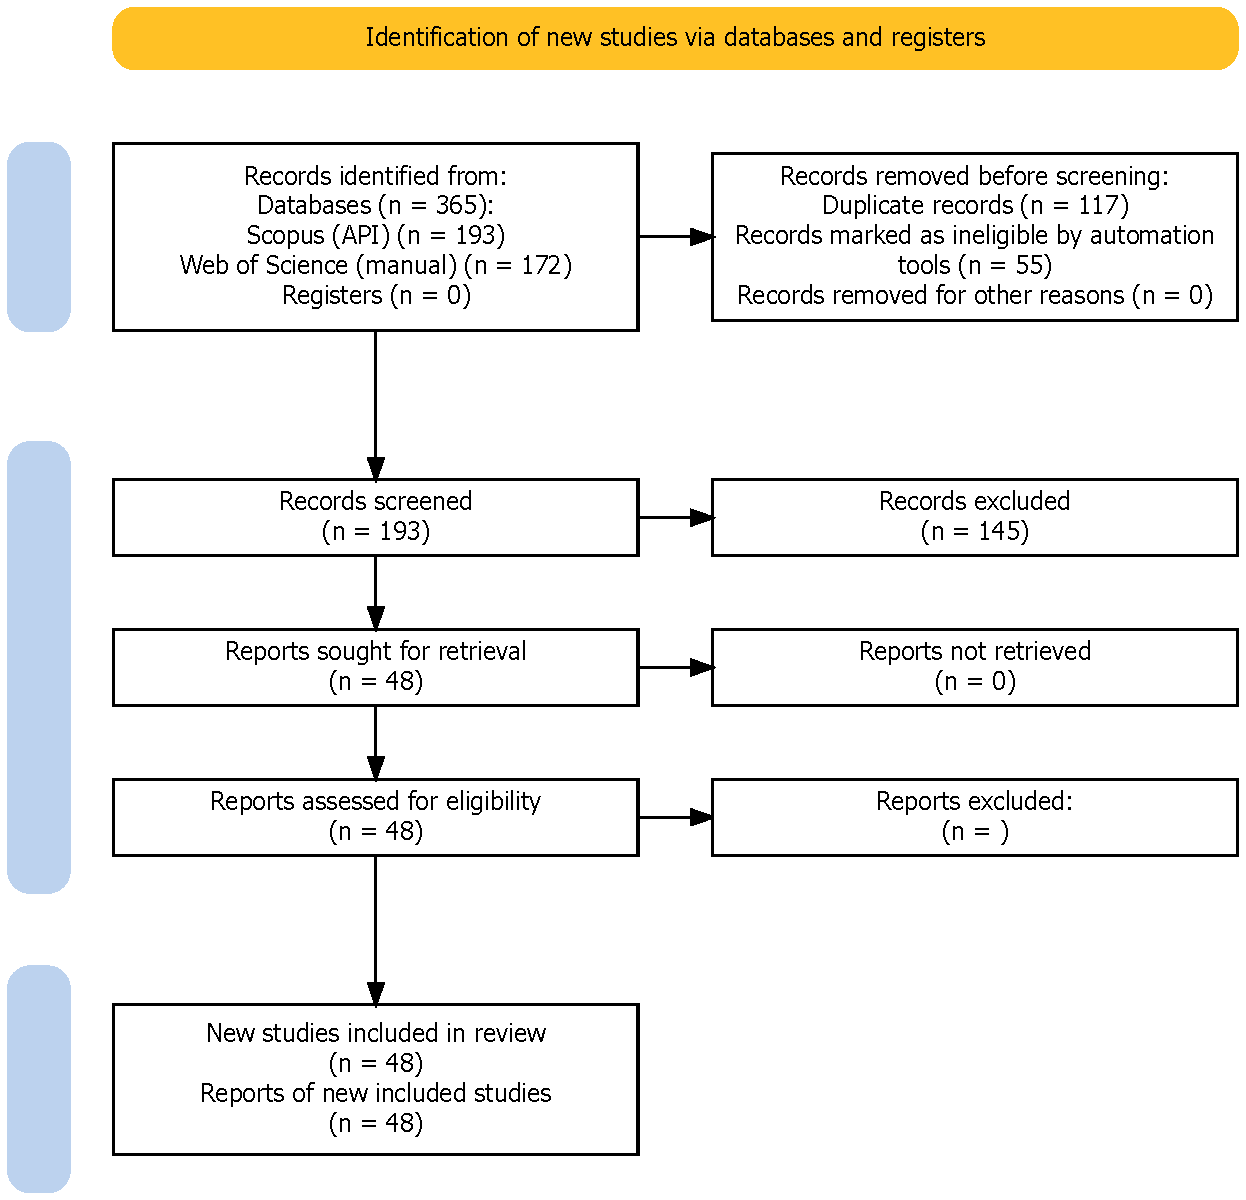
\includegraphics[width=0.88\textwidth]{3-FIGURAS/prisma_flowdiagram_artigo2_en.pdf}
\caption{PRISMA 2020 flow diagram mapping the systematic search in the Scopus and Web of Science Core Collection databases, screening restrictions, and deduplication across databases.}
\label{fig:prisma-flow}
\end{figure}

\newpage

%% ============================================================
%% S2. Meta-analysis results by dimension
%% ============================================================
\section{Meta-analysis results by dimension}
\label{app:tabela}

\begin{table}[H]
\caption{Meta-analysis results by biocultural vulnerability dimension ($k = 37$ studies per dimension, \texttt{rma.mv} model with REML and RVE-CR2, $\rho = 0.8$).}
\label{tab:meta-results}
\centering
\small
\begin{tabular}{lrrrrrr}
\toprule
\textbf{Dimension} & $\overline{lnRR}$ & \textbf{SE} & \textbf{95\% CI} & $\tau^2$ & $I^2$ (\%) & \textbf{Var. \%} \\
\midrule
$V_1$ Intergenerational Erosion    & $-0.017$ & 0.108 & $[-0.24;\; 0.21]$ & 0.169 & 14.8 & $-1.7$ \\
$V_2$ Biocultural Complexity       & $+0.045$ & 0.051 & $[-0.07;\; 0.16]$ & 0.021 &  2.4 & $+4.6$ \\
$V_3$ Territorial Uniqueness       & $+0.072$ & 0.074 & $[-0.09;\; 0.23]$ & 0.028 &  6.1 & $+7.4$ \\
$V_4$ Documentation Status         & $+0.007$ & 0.102 & $[-0.21;\; 0.22]$ & 0.093 &  7.6 & $+0.7$ \\
\textbf{$V_5$ Legal Vulnerability} & $\mathbf{-0.279}$ & \textbf{0.105} & $\mathbf{[-0.49;\; -0.06]}$ & \textbf{0.171} & \textbf{30.7} & $\mathbf{-24.3}$ \\
$V_6$ Social Organization          & $+0.172$ & 0.106 & $[-0.05;\; 0.40]$ & 0.101 &  8.4 & $+18.7$ \\
\bottomrule
\end{tabular}
\begin{flushleft}
\footnotesize \textit{Notes:} SE = robust standard error (CR2). Var.~\% = $(e^{lnRR} - 1) \times 100$.  CI in bold indicates $p < 0.05$.
\end{flushleft}
\end{table}

\newpage

%% ============================================================
%% S3. Indicator-to-dimension mapping
%% ============================================================
\section{Indicator-to-dimension mapping}
\label{app:mapping}

\begin{table}[H]
\caption{Mapping between meta-analytic indicators and functional dimensions of biocultural vulnerability.}
\label{tab:mapping}
\centering
\small
\begin{tabular}{p{0.8cm}p{2.0cm}p{3.5cm}p{2.5cm}p{3.0cm}}
\toprule
\textbf{Dim.} & \textbf{Designation} & \textbf{Meta-analytic indicator ($lnRR$)} & \textbf{Functional variable} & \textbf{Evidence status} \\
\midrule
$V_1$ & Intergener. Erosion & $\overline{lnRR}_{V_1}$, 95\% CI & Risk of transmission discontinuity & Confirmatory ($k = 37$) \\
$V_2$ & Complexity & $\overline{lnRR}_{V_2}$, 95\% CI & Biocultural density & Confirmatory ($k = 37$) \\
$V_3$ & Uniqueness & $\overline{lnRR}_{V_3}$, 95\% CI & Territorial exclusivity & Confirmatory ($k = 37$); restricted Tier~1 base \\
$V_4$ & Documentation & $\overline{lnRR}_{V_4}$, 95\% CI & Degree of formal registration & Confirmatory ($k = 37$); contextual moderators \\
$V_5$ & Legal Vuln. & $\overline{lnRR}_{V_5}$, 95\% CI & Exposure to misappropriation & Confirmatory ($k = 37$); restricted Tier~1 base \\
$V_6$ & Social Org. & $\overline{lnRR}_{V_6}$, 95\% CI & Organizational vitality & Confirmatory ($k = 37$) \\
\bottomrule
\end{tabular}
\end{table}

\newpage

%% ============================================================
%% S4. Evidence availability diagnosis
%% ============================================================
\section{Evidence availability diagnosis}
\label{app:viability}

\begin{table}[H]
\caption{Evidence availability diagnosis and analytical strategy by vulnerability dimension.}
\label{tab:viability}
\centering
\small
\begin{tabular}{p{0.8cm}p{2.2cm}p{1.2cm}p{2.0cm}p{5.5cm}}
\toprule
\textbf{Dim.} & \textbf{Designation} & \textbf{$k$} & \textbf{Status} & \textbf{Analytical strategy} \\
\midrule
$V_1$ & Intergener. Erosion & 37 & Confirmatory & Full meta-analysis (forest plot, meta-regression, publication bias) \\
$V_2$ & Complexity & 37 & Confirmatory & Full meta-analysis \\
$V_3$ & Uniqueness & 37 & Confirmatory & Full meta-analysis; restricted Tier~1 base, interpret with caution \\
$V_4$ & Documentation & 37 & Confirmatory & Full meta-analysis; meta-regression with moderators \\
$V_5$ & Legal Vuln. & 37 & Confirmatory & Full meta-analysis; restricted Tier~1 base, interpret with caution \\
$V_6$ & Social Org. & 37 & Confirmatory & Full meta-analysis; meta-regression with moderators \\
\bottomrule
\end{tabular}
\end{table}

\end{document}
